\documentclass[12pt,letterpaper]{article}
\usepackage[latin1]{inputenc}
\usepackage{amsmath}
\usepackage{amsfonts}
\usepackage{amssymb}
\usepackage{graphicx}

\graphicspath{{./plots/}}
\begin{document}
\title{GDD Project \\ \vspace{.5 cm} {\Large Computer Based Course and Application Tools Project} }
\author{Please add your name~Farhad M. Kazemi ~ Please add your name}
\maketitle
\begin{abstract}
The aim of this research is to find the...

The results showed that...
\end{abstract}

\section{Introduction}

In this report, we would like to...

On the rest of this report, firstly we will describe our dataset properties and what we have done to clean this data and to overcome data heterogeneity and missing values. In the second section, we briefly described ....
Finally, we have a conclusion and what could be done in the future works.
\subsection{Dealing With Dataset}
The dataset consists of 

The input dataset has 
\begin{enumerate}
\item \textbf{G:} We used this method for imputing missing data and extracting features on raw data (... sample with features). More details are available in section 2.
\end{enumerate}
\noindent Because of our time limit and for avoiding further complexity, we only considered 3 datasets which are ... 
It means we have datasets with ... samples and ... features respectively. Table shows the datasets and their number of samples.
\section{Methods}
In this section, we will describe principles of methods that we used for analyzing data. We will explain a ... as well as ....  Furthermore, we will describe .... 
\subsection{ section}

<<<<<<< HEAD
\section{Question 1}
\section{Question 2}
\section{Question 3}
Write a command line program that takes arguments.\\
\section{Question 4}
\section{Question 5}
\section{Question 6}
\section{Question 7}
\section{Question 8}
\section{Question 9}
\section{Question 10}
\section{Question 1 optional}
\section{Question 2 optional}
\section{Question 3 optional}
=======
\section{Question 3}
Write a command line program that takes arguments\\
\begin{figure}
\centering
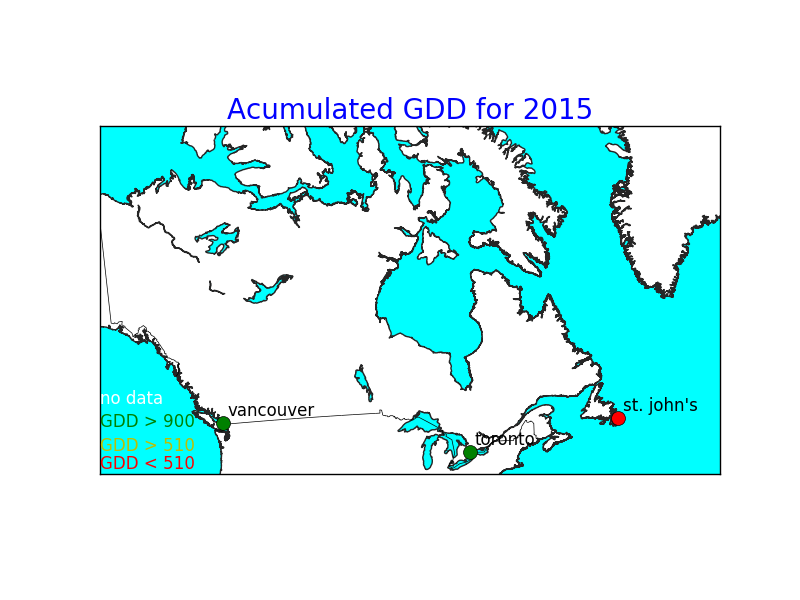
\includegraphics[scale=0.6]{GDDMap_2015.png}
\caption{F}
\end{figure}

\begin{figure}
\centering
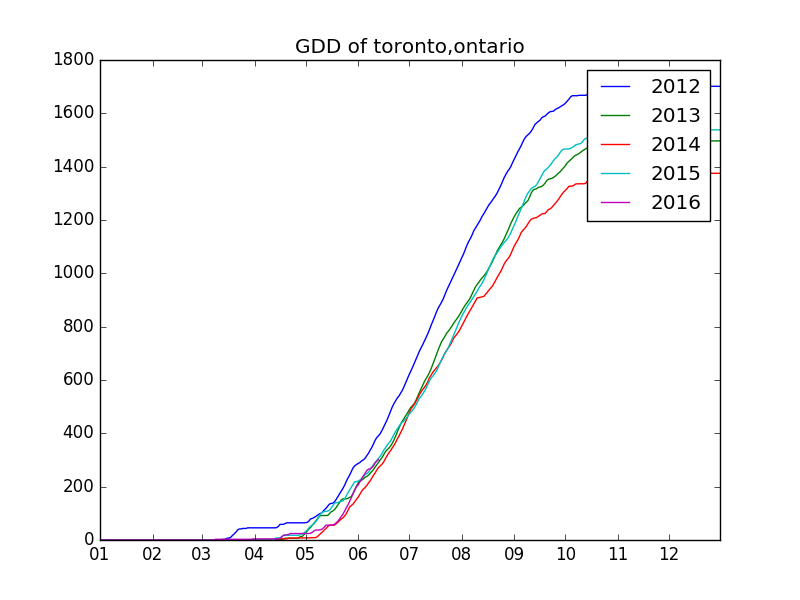
\includegraphics[scale=0.6]{toronto,ontario_GddPlot.png}
\caption{B}
\label{fig:gbm}
\end{figure}

\begin{figure}
\centering
\includegraphics[scale=0.6]{{"st. john's,newfoundland_GddPlot"}.png}
\caption{A}
\label{fig:gbm}
\end{figure}

\begin{figure}
\centering
\includegraphics[scale=0.6]{{"vancouver,british columbia_GddPlot"}.png}
\caption{C}
\end{figure}

\begin{figure}
\centering
\includegraphics[scale=0.6]{{"st. john's,newfoundland_MinMax"}.png}
\caption{D}
\end{figure}

\begin{figure}
\centering
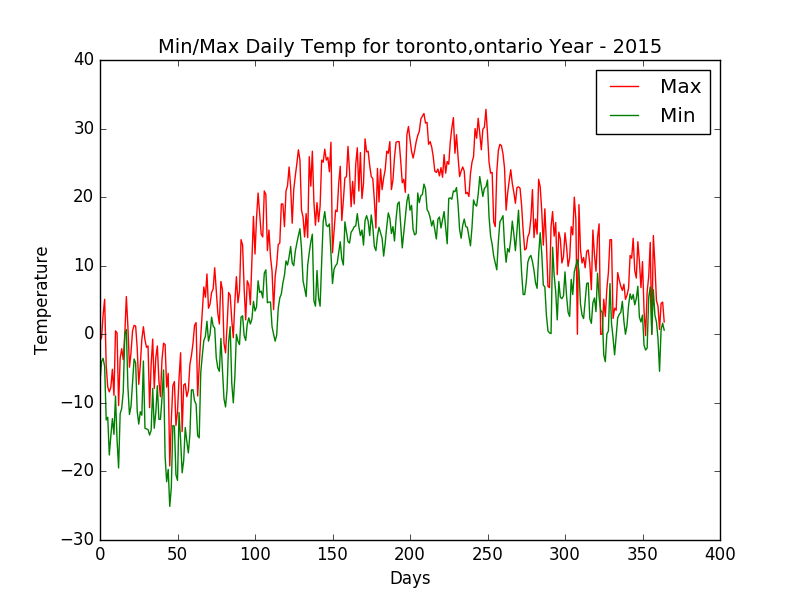
\includegraphics[scale=0.6]{toronto,ontario_MinMax.png}
\caption{E}
\end{figure}

\begin{figure}
\centering
\includegraphics[scale=0.6]{{"vancouver,british columbia_MinMax"}.png}
\caption{F}
\end{figure}


%\includegraphics{plot00.png}
%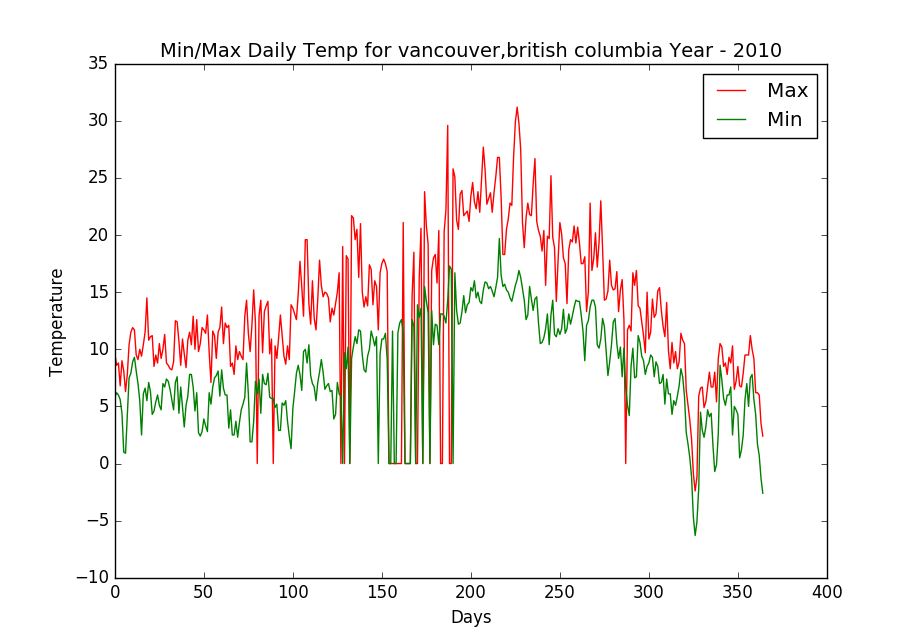
\includegraphics{Plot01.png}
%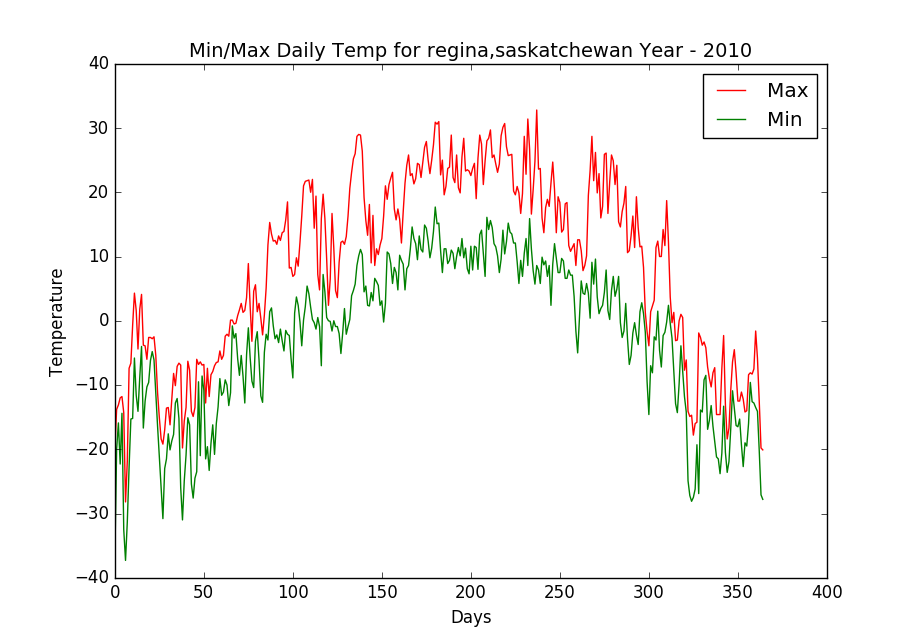
\includegraphics{Plot02.png}
%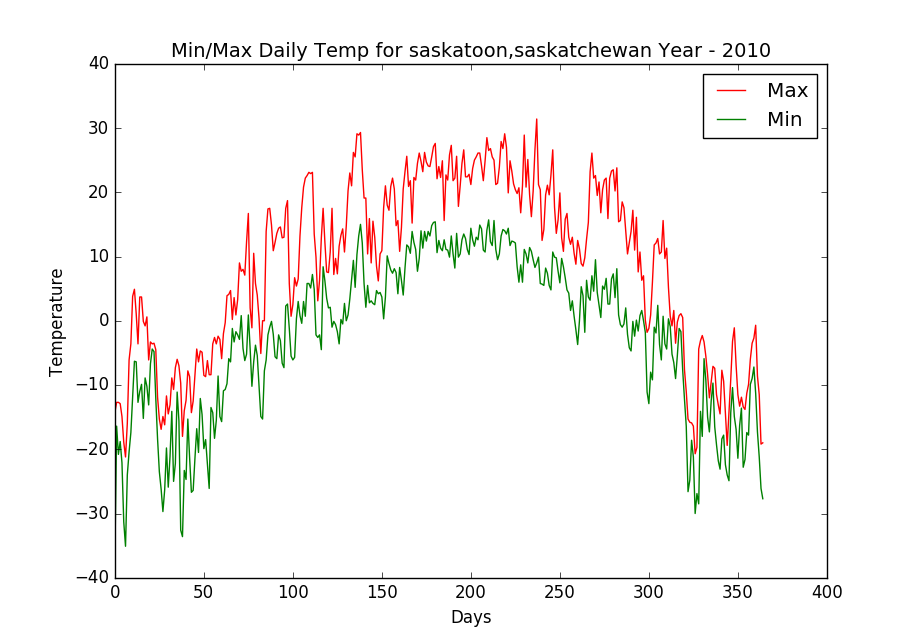
\includegraphics{Plot03.png}
%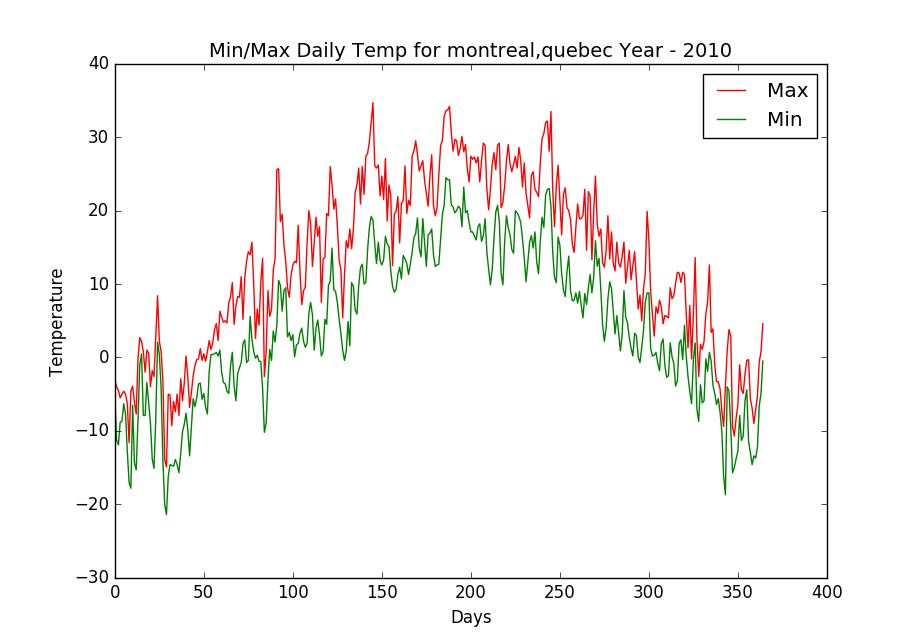
\includegraphics{Plot04.png}
%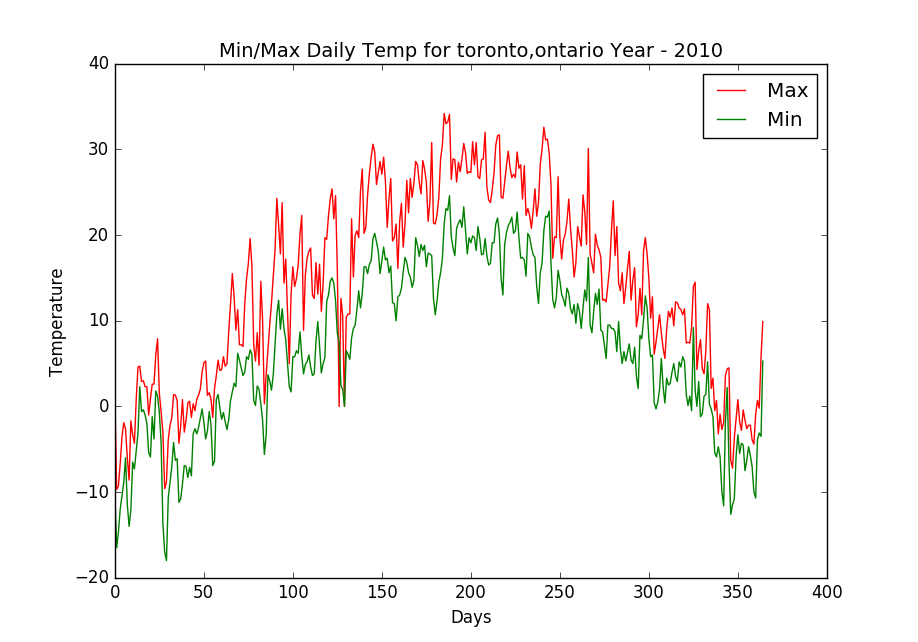
\includegraphics{Plot05.png}
\subsubsection{section}
\section{Experimental Results}
In our experiments, we used 
\subsection{result}
Parameter settings listed in table 1 was used for exploring the performance of 
\section{Discussion}
\section{Conclusion}
In this work ...
\newpage
\end{document}
